%-----------------------------------------------------------------------------%
%	Packages & Other Configurations
%-----------------------------------------------------------------------------%
\RequirePackage{fix-cm}  % Fix Font shape `OT1/cmr/m/n' size substitution.
\documentclass[a4paper,10pt]{article}
\usepackage[top=0.3in, bottom=0.3in, left=1in, right=0.9in]{geometry}
\usepackage[utf8]{inputenc} %add acents
\usepackage{setspace} % command \doublespacing etc...
\usepackage{lineno} % number lines
\usepackage{epsf,epsfig} % includegraphics [pdf, png etc]
\usepackage{amsmath} %adicionei esse pacote pra vc poder usar o draft%
\usepackage{textcomp} %símbolos de texto
\usepackage{natbib} % bibtex - adicionar referencia
% \usepackage{url} % for bibtex - configuracoes de urls
\usepackage{tabularx} % for tables
\usepackage[hidelinks]{hyperref}  % Add URL links.
% \usepackage[bookmarks=false,colorlinks=true,urlcolor={green},linkcolor={green},pdfstartview={XYZ null null 1.22}]{hyperref} %all references
\usepackage{tikz}
\usepackage{lscape}
\usepackage{siunitx}
\usepackage{geometry}

%-----------------------------------------------------------------------------%
%	Adicionar a Watermark
%-----------------------------------------------------------------------------%
\usepackage{draftwatermark}
\SetWatermarkAngle{45}
\SetWatermarkLightness{0.9}
\SetWatermarkFontSize{5cm}
\SetWatermarkScale{0.3}
\SetWatermarkText{Prática 1 - Oceanografia}

%-----------------------------------------------------------------------------%
%	Informações sobre o PDF
%-----------------------------------------------------------------------------%
\pdfinfo{%
  /Title    (GEO232 - Prática 1)
  /Author   (Ju Leonel)
  /Creator  (Ju Leonel)
  /Producer (Ju Leonel)
  /Subject  (Intro oceanografias)
  /Keywords (Intro oceanografia, prática 1)}

%-----------------------------------------------------------------------------%
%	Documento
%-----------------------------------------------------------------------------%
\title{GEO232 - Introdução à Oceanografia - IGEO-UFBA}
\author{\vspace{-10ex}}
\date{\vspace{-10ex}}

\geometry{hmargin=0.5cm,vmargin=0.5cm}

\def\width{25}
\def\hauteur{4}

\begin{document}
\begin{landscape}

  \maketitle
  %\doublespacing
  %\onehalfspace
  %\phantom{}

  \vspace{0.5 cm}

    \begin{center}
    \begin{tabular}{l r r}
      \multicolumn{3}{l}{\Large{Batimetria do Oceano Atlântico Norte a 31\si{\degree}}} \\
      \hline
                                        & \multicolumn{1}{l}{{\bf Distância}}         & \multicolumn{1}{l}{{\bf Profundidade}}     \\
              {\bf Feição Topográfica} & \multicolumn{1}{l}{{\bf (Milhas Náuticas)}} & \multicolumn{1}{l}{{\bf (Braças)}} \\
      \hline
      \multicolumn{3}{l}{\phantom{}} \\
    Costa da Flórida                    &    0  &    0  \\
    Plataforma Continental da Flórida   &   95  &  100  \\
                                        &  250  & 1000  \\
                                        &  315  & 2000  \\
                                        &  375  & 2450  \\
    Blake Outer Ridge                   &  565  & 2200  \\
    Planície Abissal Hatteras           &  755  & 2850  \\
    Elevado de Bermuda                  & 1040  & 2700  \\
    Bacia Norte-Americana               & 1130  & 3000  \\
    Cordilheira Meso-Oceânica           & 2610  & 2000  \\
                                        & 2765  & 1810  \\
                                        & 3020  & 2000  \\
    Planície Abissal Cape Verde         & 3835  & 3000  \\
                                        & 3900  & 3440  \\
                                        & 3960  & 3000  \\
                                        & 4465  & 2000  \\
    Plataforma Continental de Marrocos  & 4840  & 1000  \\
                                        & 4900  &  100  \\
    Costa de Marrocos                   & 4935  &    0  \\
      \hline
    \end{tabular}
    \end{center}

%\vspace{1cm}

  \begin{center}
  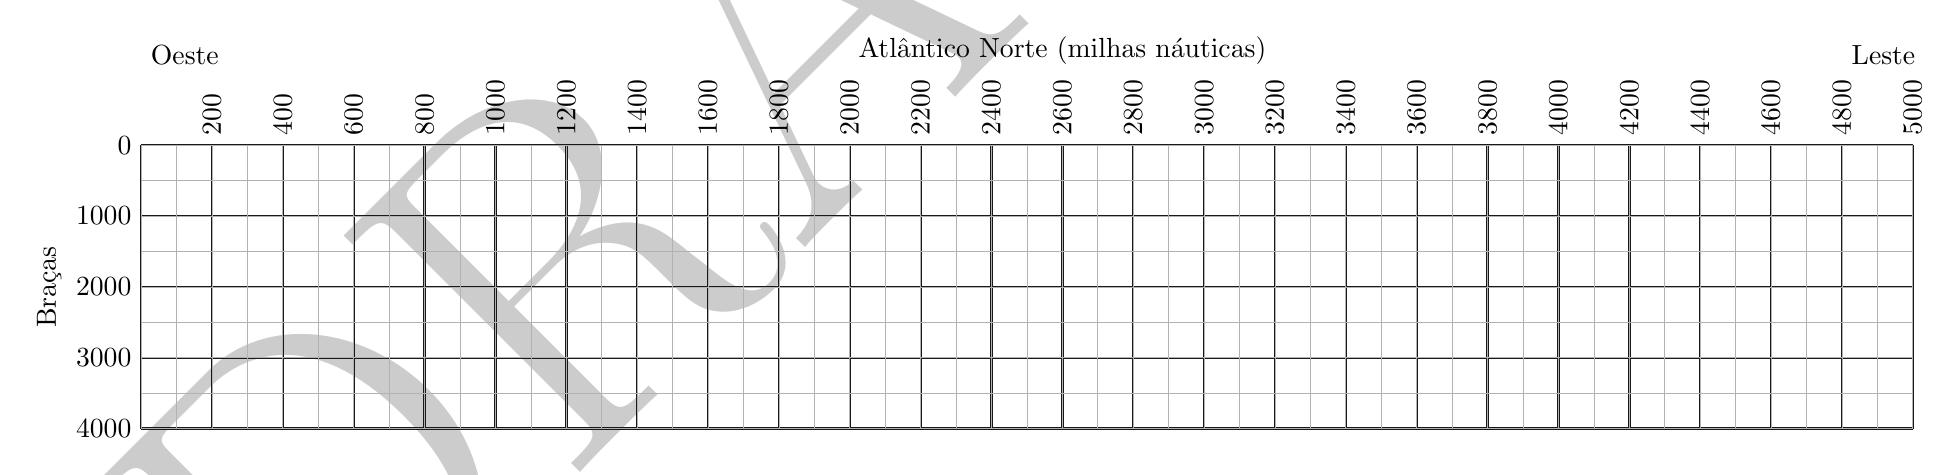
\begin{tikzpicture}[x=0.90cm, y=0.90cm]
    % Grid.
    \draw[step=0.90cm, line width=0.3mm, black!90!white] (0,0) grid (\width,\hauteur);
    \draw[step=0.45cm, line width=0.1mm, black!30!white] (0,0) grid (\width,\hauteur);
    % y-label.
    \draw[black] (-1, 2) node[anchor=south, rotate=90] {Braças};
    % y-tickslabels.
    \draw[black] (0, 4) node[anchor=east] {0};
    \draw[black] (0, 3) node[anchor=east] {1000};
    \draw[black] (0, 2) node[anchor=east] {2000};
    \draw[black] (0, 1) node[anchor=east] {3000};
    \draw[black] (0, 0) node[anchor=east] {4000};
    % x-labels.
    \draw[black] ( 0, 5) node[anchor=south west] {Oeste};
    \draw[black] (24, 5) node[anchor=south west] {Leste};
    \draw[black] (13, 5) node[anchor=south] {Atlântico Norte (milhas náuticas)};
    % x-tickslabels.
    \draw[black] ( 1, 4) node[anchor=west, rotate=90] {200};
    \draw[black] ( 2, 4) node[anchor=west, rotate=90] {400};
    \draw[black] ( 3, 4) node[anchor=west, rotate=90] {600};
    \draw[black] ( 4, 4) node[anchor=west, rotate=90] {800};
    \draw[black] ( 5, 4) node[anchor=west, rotate=90] {1000};
    \draw[black] ( 6, 4) node[anchor=west, rotate=90] {1200};
    \draw[black] ( 7, 4) node[anchor=west, rotate=90] {1400};
    \draw[black] ( 8, 4) node[anchor=west, rotate=90] {1600};
    \draw[black] ( 9, 4) node[anchor=west, rotate=90] {1800};
    \draw[black] (10, 4) node[anchor=west, rotate=90] {2000};
    \draw[black] (11, 4) node[anchor=west, rotate=90] {2200};
    \draw[black] (12, 4) node[anchor=west, rotate=90] {2400};
    \draw[black] (13, 4) node[anchor=west, rotate=90] {2600};
    \draw[black] (14, 4) node[anchor=west, rotate=90] {2800};
    \draw[black] (15, 4) node[anchor=west, rotate=90] {3000};
    \draw[black] (16, 4) node[anchor=west, rotate=90] {3200};
    \draw[black] (17, 4) node[anchor=west, rotate=90] {3400};
    \draw[black] (18, 4) node[anchor=west, rotate=90] {3600};
    \draw[black] (19, 4) node[anchor=west, rotate=90] {3800};
    \draw[black] (20, 4) node[anchor=west, rotate=90] {4000};
    \draw[black] (21, 4) node[anchor=west, rotate=90] {4200};
    \draw[black] (22, 4) node[anchor=west, rotate=90] {4400};
    \draw[black] (23, 4) node[anchor=west, rotate=90] {4600};
    \draw[black] (24, 4) node[anchor=west, rotate=90] {4800};
    \draw[black] (25, 4) node[anchor=west, rotate=90] {5000};
  \end{tikzpicture}
  \end{center}

\end{landscape}
\end{document}  
  